\documentclass[tikz,border=2pt,11pt]{standalone}
\usetikzlibrary{arrows.meta}
\usetikzlibrary{calc}
\usetikzlibrary{fit}
\usetikzlibrary{positioning}
\usepackage{amsmath}
\usepackage{amssymb}
\usepackage{graphicx}
\usepackage{xcolor}
\usepackage{tikz}
\newcommand{\R}{\mathbb R}
\newcommand{\N}{\mathbb N}
\newcommand{\Z}{\mathbb Z}
\newcommand{\dd}{\mathrm d}
\newcommand{\eps}{\varepsilon}
\newcommand{\cD}{\mathcal D}
\newcommand{\cA}{\mathcal A}
\newcommand{\cT}{\mathcal T}
\newcommand{\cP}{\mathcal P}
\newcommand{\cL}{\mathcal L}
\newcommand{\KN}{Kerr--Newman}
\DeclareMathOperator{\tr}{tr}
\DeclareMathOperator{\divg}{div}
\DeclareMathOperator{\Ric}{Ric}
\DeclareMathOperator{\Hess}{Hess}
\DeclareMathOperator{\supp}{supp}
\DeclareMathOperator{\dist}{dist}
\DeclareMathOperator{\Area}{Area}
\DeclareMathOperator{\Vol}{Vol}
\DeclareMathOperator{\id}{id}
\DeclareMathOperator{\sgn}{sgn}
\begin{document}
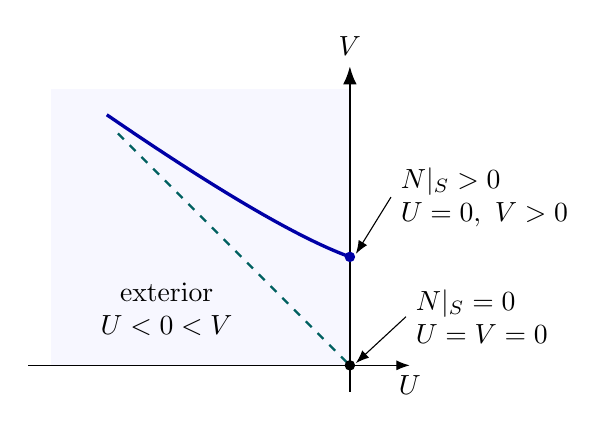
\begin{tikzpicture}[scale=0.95,>=Latex]
  \fill[blue!3] (-4,0) rectangle (0,3.7);
  \draw[->] (-4.3,0)--(0.8,0) node[below] {\(U\)};
  \draw[->,thick] (0,-0.35)--(0,4.0) node[above] {\(V\)};
  \draw[very thick,blue!65!black]
      (-3.25,3.35) .. controls (-1.5,2.15) and (-0.55,1.65)
                   .. (0,1.45);
  \draw[thick,dashed,teal!75!black] (-3.1,3.1)--(0,0);
  \fill[blue!65!black] (0,1.45) circle (2pt);
  \fill (0,0) circle (2pt);
  \node[align=left,anchor=west] (future) at (0.55,2.25)
      {\(N|_S>0\)\\\(U=0,\ V>0\)};
  \draw[->] (future.west)--(0.08,1.49);
  \node[align=left,anchor=west] (bif) at (0.75,0.65)
      {\(N|_S=0\)\\\(U=V=0\)};
  \draw[->] (bif.west)--(0.08,0.03);
  \node[align=center] at (-2.45,0.75)
      {exterior\\\(U<0<V\)};
 \end{tikzpicture}
\end{document}
